\documentclass[11pt]{article}
\usepackage[a4paper,margin=2.2cm]{geometry}
\usepackage{amsmath,amssymb}
\usepackage{xcolor}
\usepackage{booktabs}
\usepackage{enumitem}
\usepackage[most]{tcolorbox}
\usepackage{tikz}
\usetikzlibrary{arrows.meta,positioning,shapes.geometric,calc}
\usepackage{hyperref}
\hypersetup{colorlinks=true,linkcolor=blue!55!black,urlcolor=blue!55!black}

\definecolor{ink}{HTML}{1b2430}
\definecolor{accent}{HTML}{234e70}
\definecolor{soft}{HTML}{eef3f7}
\definecolor{good}{HTML}{1f7a4d}

\newtcolorbox{keybox}[1][]{colback=soft,colframe=accent,boxrule=0.6pt,
  arc=2pt,left=6pt,right=6pt,top=5pt,bottom=5pt,fonttitle=\bfseries,title=#1}
\newtcolorbox{notebox}[1][]{colback=white,colframe=good,boxrule=0.6pt,
  arc=2pt,left=6pt,right=6pt,top=4pt,bottom=4pt,fonttitle=\bfseries,title=#1}

\setlist{nosep,leftmargin=1.2em}
\newcommand{\gf}{\mathrm{GF}(256)}
\newcommand{\hw}{\mathrm{HW}}
\newcommand{\xor}{\oplus}
\color{ink}

\title{\vspace{-1.2cm}\textbf{Recovering the MQOM v2.1 Secret Key by CPA}\\[2pt]
\large A short study guide --- how the attack works, not all of MQOM}
\author{BTP: Side-Channel CPA Analysis of MQOM v2.1}
\date{\today}

\begin{document}
\maketitle
\vspace{-0.6cm}

\begin{notebox}[Scope of this note]
This explains \emph{how we recover the secret key}, with the minimum MQOM background
needed. It deliberately does \textbf{not} explain the full MQOM signature scheme. Every
result here is a \textbf{computer simulation} under stated leakage models --- a property
of the models, \emph{not} a demonstrated weakness of any real device.
\end{notebox}

\section*{1\quad The 60-second picture}
The secret key is a vector $x$ of \textbf{48 bytes} over the byte-field $\gf$ (the AES
field). We recover it in three moves:
\begin{enumerate}
\item Split $x$ into a \textbf{prefix} (first 16 bytes) and a \textbf{suffix} (last 32 bytes).
\item Recover each half separately with \textbf{CPA} (a side-channel guessing method), using
two different moments in the signing computation.
\item Stitch the halves together and \textbf{confirm} the full key with MQOM's public equations.
\end{enumerate}

\begin{center}
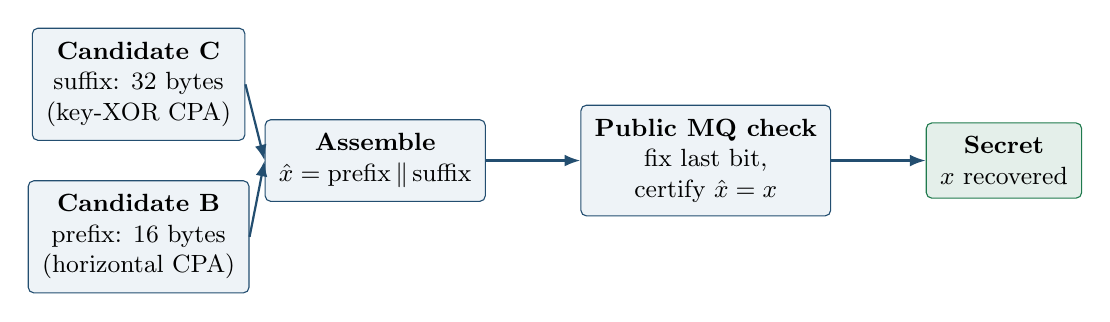
\begin{tikzpicture}[font=\small,node distance=6mm,
  box/.style={draw=accent,fill=soft,rounded corners=2pt,inner sep=5pt,align=center,minimum height=9mm},
  arr/.style={-{Latex[length=2mm]},accent,thick}]
\node[box] (c) {\textbf{Candidate C}\\suffix: 32 bytes\\(key-XOR CPA)};
\node[box,below=5mm of c] (b) {\textbf{Candidate B}\\prefix: 16 bytes\\(horizontal CPA)};
\node[box,right=16mm of $(c)!0.5!(b)$] (asm) {\textbf{Assemble}\\$\hat{x}=\text{prefix}\,\Vert\,\text{suffix}$};
\node[box,right=12mm of asm] (mq) {\textbf{Public MQ check}\\fix last bit,\\certify $\hat x=x$};
\node[box,right=12mm of mq,fill=good!12,draw=good] (x) {\textbf{Secret}\\$x$ recovered};
\draw[arr] (c.east) -- (asm.west);
\draw[arr] (b.east) -- (asm.west);
\draw[arr] (asm) -- (mq);
\draw[arr] (mq) -- (x);
\end{tikzpicture}
\end{center}

\section*{2\quad The minimum MQOM you need}
Four facts are enough to follow the attack:
\begin{itemize}
\item \textbf{The key.} The secret witness $x\in\gf^{48}$ --- 48 bytes we want to find.
\item \textbf{The public equations.} MQOM's public key fixes a quadratic system and its value
at the secret:
\[
 y_i \;=\; x^{\!\top} A_i\,x \;+\; b_i^{\!\top} x,\qquad i=1,\dots,48,
\]
with all $A_i,b_i,y$ \textbf{public}. We only use this at the very end, as a check.
\item \textbf{Where $x$ leaks.} While signing, $x$ is combined with public and random values.
Two such moments each expose part of $x$ to analysis --- one for the suffix, one for the
prefix. That is all we need from the signing algorithm.
\item \textbf{The leakage model.} We assume the device's power/EM signal grows with the
\textbf{Hamming weight} $\hw(v)$ (the number of 1-bits) of the byte $v$ it is handling. This
is the standard, realistic assumption. In simulation: $\;L=\hw(v)+\text{noise}$.
\end{itemize}

\begin{keybox}[CPA in one line]
\textbf{Correlation Power Analysis.} A fixed secret byte meets \emph{known, varying} data.
For each guess $g\in\{0,\dots,255\}$ we predict the Hamming weight of an intermediate value,
and correlate the prediction against the measured leakage $L$ over many samples:
\[
 \rho(g)=\mathrm{corr}\big(\,L,\ \hw(\text{intermediate}(g))\,\big),\qquad
 \hat{x}= \arg\max_g |\rho(g)|.
\]
The correct guess lines up with the real leakage and gives the peak correlation.
\end{keybox}

\section*{3\quad Suffix (32 bytes) --- Candidate C}
When signing, the key is blended with a random share sum $\mathrm{acc}$, producing a
correction $\Delta = x \xor \mathrm{acc}$. For the \textbf{suffix} bytes, $\Delta$ is
\emph{published in the signature} and changes every signature, while the secret operand
$\mathrm{acc}$ is what leaks. Since
\[
 \mathrm{acc}[k] \;=\; x[k]\,\xor\,\Delta[k],
\]
this is the textbook \textbf{key-XOR CPA}: $\Delta[k]$ is the known varying data, and we guess
$x[k]$ by predicting $\hw\big(g \xor \Delta[k]\big)$ and correlating across signatures.

\begin{itemize}
\item \textbf{One subtlety.} For an XOR target, a byte and its bit-flip (complement) look
identical to $|\rho|$. Using the \emph{signed} correlation separates them, leaving just a
single global $\pm$ sign for the whole suffix --- fixed later by the public equations.
\item \textbf{Outcome.} All 32 suffix bytes, from a few hundred signatures at realistic noise.
\end{itemize}

\section*{4\quad Prefix (16 bytes) --- Candidate B}
The suffix trick cannot reach the prefix (there $\Delta=0$, no varying public data). We use a
different moment: the signer computes a matrix--vector product $t = A\,x$, in which each secret
byte $x_j$ is multiplied by \textbf{many public numbers} $a$ \emph{within a single signing}.
That gives a ``horizontal'' axis of known varying data:
\[
 \text{for many positions: leakage of } x_j\cdot a,\qquad
 \rho(g)=\mathrm{corr}_{\text{positions}}\big(L,\ \hw(g\cdot a)\big).
\]

\begin{itemize}
\item \textbf{Why it is clean.} Multiplying by a fixed $a$ is a one-to-one map, so the correct
guess is the unique peak. A wrong guess $g$ only correlates through $c=g\cdot x_j^{-1}$, and
no $c\neq 1$ mimics the truth --- so there is \emph{no} complement ambiguity here.
\item \textbf{One blind spot.} If $x_j=0$ then $x_j\cdot a=0$ for every $a$: the channel is
dead and that byte cannot be read this way. But we \textbf{detect} it (the peak collapses to
noise), so it is never a silent error --- the public equations fill it in (Section 6).
\item \textbf{Backup (Candidate F).} A second-order trick on the seed tree. Under the realistic
model it only reveals each byte's \emph{Hamming weight}, not the byte --- so it stays a backup,
never the main route.
\item \textbf{Outcome.} All 16 prefix bytes (bar a detectable zero), robust to noise.
\end{itemize}

\section*{5\quad Assemble + certify (Part 3)}
Now $\hat x = \text{prefix}\,\Vert\,\text{suffix}$, with two small leftovers: the suffix's
global $\pm$ sign, and any detected zero byte. We resolve both with the \textbf{public MQ
equations} from Section 2, used \emph{only as a check}:

\begin{itemize}
\item The true key satisfies all 48 equations $y_i = \hat x^{\!\top}A_i\hat x + b_i^{\!\top}\hat x$;
a key wrong in even one byte fails essentially all of them (a sharp test).
\item So we try the two sign options (and brute-fill a rare zero byte), and keep the one
assignment that satisfies every equation. That \textbf{certifies} $\hat x = x$.
\end{itemize}

\begin{keybox}[The golden rule of this project]
CPA does the \textbf{recovery}; the algebra only \textbf{combines, completes and verifies}.
The equations are never used to \emph{solve} for the key --- only to pick the last bit, fill a
detected gap, and prove the answer is right.
\end{keybox}

\section*{6\quad Does it work?}
\begin{center}\small
\begin{tabular}{@{}lll@{}}
\toprule
Step & What is recovered & Result (simulation) \\
\midrule
Candidate C & 32 suffix bytes & 100\% at realistic noise \\
Candidate B & 16 prefix bytes & 100\% of non-zero bytes; zeros detected \\
Assemble + MQ check & full 48-byte key & $\hat x = x$, 100\%, zero false accepts \\
\bottomrule
\end{tabular}
\end{center}

\noindent The pipeline was \textbf{independently audited}: the field math, the correlation
code and the equations were re-derived and re-run from scratch, and a specific check confirmed
the attacker never sees the key (removing the real signal drops recovery to chance). Honest
scope: these are synthetic demonstrations under a stated leakage model, not a break of any real
MQOM implementation.

\clearpage
\begin{center}
{\Large\bfseries Part II --- Defence Pack}\\[2pt]
\small\textit{Extra depth for the viva: the proofs, the numbers, the limits, and the
cross-questions a panel is likely to ask.}
\end{center}
\vspace{2mm}

\section*{7\quad A bit more MQOM (only what the panel will probe)}
The primer said ``$x$ leaks at two moments.'' Here is \emph{why}, because a panel will ask
why the prefix and suffix are attacked differently.

\begin{itemize}
\item \textbf{The split is not our choice --- MQOM exposes the two halves differently.}
The signer forms the correction $\Delta = x \xor \mathrm{acc}$ (acc = sum of fresh random
shares). Only the \textbf{suffix} part $\Delta[16{:}48]$ is \emph{serialised into the public
signature}; it varies every signature. That public, varying value is exactly the handle
Candidate~C needs.
\item \textbf{Why the prefix has no such handle.} The first 16 bytes
$\delta=\mathrm{FirstBits}(x)=x[0{:}16]$ are not published as a correction --- they are fed
into the \textbf{correlated seed tree} as $\text{node}_3=\text{rseed}\xor\delta$ (rseed =
fresh random mask). So on the prefix, $\Delta=0$: no public varying data $\Rightarrow$
Candidate~C is blind there. That is the whole reason we need a second route.
\item \textbf{The two leak points, precisely.}
(i)~Candidate~C/F feed on the sharing step; (ii)~Candidate~B feeds on
$t = \hat A\,x$ (public matrix $\times$ secret), computed every signature, where each $x_j$
meets many public coefficients.
\end{itemize}

\section*{8\quad Anticipated panel cross-questions}

\subsection*{8.1\quad Method and model}
\begin{itemize}
\item \textbf{\textit{Q: Why CPA, and not DPA / template / SASCA?}}\\
A: CPA needs no device profiling and only a weak leakage assumption (power grows with
Hamming weight), so it is the most portable and falsifiable choice --- and it is the mandated
mechanism for this project. DPA is essentially a special case; template and SASCA are
\emph{stronger}-assumption attacks (they need a profiling phase or a full factor graph), which
we deliberately avoid so the result rests on as little as possible.
\item \textbf{\textit{Q: Is the Hamming-weight leakage model realistic?}}\\
A: Yes --- on CMOS, dynamic power tracks the number of switching bits, so HW (and weighted-HW)
is the standard first-order model. We also test \emph{mismatch}: the attacker always predicts
plain HW while the ``device'' leaks weighted-HW; recovery survives. The only shape that breaks
it is a \emph{non-monotone} bit (leaking ``backwards''), which we use strictly as a labelled
stress test, never as the realistic model.
\item \textbf{\textit{Q: Why signed correlation for the suffix but absolute for the prefix?}}\\
A: The suffix target is XOR-linear, so a byte and its complement are perfectly
\emph{anti}-correlated --- the \emph{sign} carries the information, so we keep it. The prefix
target is a field \emph{multiply} (non-linear), which has no such symmetry, so $|\rho|$ is fine.
\end{itemize}

\subsection*{8.2\quad Correctness --- be ready to prove these}
\begin{itemize}
\item \textbf{\textit{Q: Prove the correct key is the unique CPA peak for the prefix.}}\\
A: With leakage $\hw(x_j a)$ and prediction $\hw(g a)$ over many public $a$, the wrong-key
correlation depends only on $c=g\,x_j^{-1}$: $\ \rho(c)=\mathrm{corr}_a(\hw(a),\hw(c\,a))$.
This equals $1$ only when $\hw(c\,a)$ is an affine function of $\hw(a)$ for all $a$, which holds
\emph{only} for $c=1$ (i.e.\ $g=x_j$). Every other $c$ gives a strictly lower peak (ceiling
$\approx 0.63$, so margin $\approx 0.37$). We confirmed this curve is key-independent in simulation.
\item \textbf{\textit{Q: Explain the suffix complement ambiguity and its fix.}}\\
A: For any affine-in-bits leakage, $g'=x\xor\texttt{0xFF}$ predicts $C-\hw(x\xor\Delta)$ ---
perfectly anti-correlated --- so $|\rho|$ ties $x$ with its complement. The \emph{signed}
correlation separates them ($+\rho$ vs $-\rho$), leaving a single \emph{global} sign bit for
the whole suffix (2 candidates), fixed by the public equations. Not $2^{32}$.
\item \textbf{\textit{Q: Why is the final MQ check trustworthy (no false accept)?}}\\
A: The system is quadratic, so one wrong byte cascades into essentially all 48 equations ---
empirically a wrong vector satisfies $\le 3/48$ and \emph{never} all 48. The chance a wrong
candidate satisfies all $m=48$ equations is $\sim 256^{-48}\approx 0$.
\end{itemize}

\subsection*{8.3\quad Integrity --- ``it's only a simulation''}
\begin{itemize}
\item \textbf{\textit{Q: It's synthetic --- what does it actually prove?}}\\
A: It proves a \emph{conditional, structural} result: \emph{if} the implementation leaks the
stated intermediates in a monotone way, \emph{then} the key is fully recoverable by CPA, and we
characterise exactly how much data and noise tolerance that takes. It is \textbf{not} a claim
that any real device leaks this way --- that would need measured traces (recommended as future
work, never performed here).
\item \textbf{\textit{Q: Isn't the MQ algebra doing the recovery, not CPA?}}\\
A: No. CPA \emph{alone} --- with the MQ step switched off --- already recovers 48/48 bytes on
40/40 keys at $\sigma=2$. The algebra only (i)~picks the global sign bit, (ii)~fills a rare
\emph{detected} zero byte, (iii)~certifies. It never \emph{solves} for a byte.
\item \textbf{\textit{Q: How do you know the simulation isn't rigged (success by construction)?}}\\
A: The distinguisher functions take only \emph{public} data and leakage --- the secret is never
an argument. Independent check: replace the real intermediate with a secret-\emph{independent}
value and recovery drops to chance; shuffle the leakage--data pairing and it collapses. An
independent audit re-derived the maths and re-ran everything and found no leakage of the key.
\end{itemize}

\subsection*{8.4\quad Numbers, cost, limits}
\begin{itemize}
\item \textbf{\textit{Q: How much data? How noise-tolerant?}}\\
A: Suffix (C): $\sim$200 signatures for 100\% at $\sigma=2$. Prefix (B): every non-zero byte at
100\% up to $\sigma=8$ with $\sim$100 averaged signatures; as few as $\sim$19 horizontal
positions suffice (single-trace needs $\sim$256--512). Full recovery is 100\% at $\sigma\le 2$;
at $\sigma=4$ the \emph{suffix} front just needs more signatures ($\sim$2000), not the assembly.
\item \textbf{\textit{Q: Cost of the algebra step?}}\\
A: Negligible: 2 polarity options, and a detected zero byte is brute-forced over 256 values
(rarely two). Each check is one evaluation of 48 quadratic equations.
\item \textbf{\textit{Q: Candidate F only gives Hamming weight --- why keep it?}}\\
A: Honesty and coverage. Under pooled HW its second-order statistic equals
$2-\hw(\delta)/2$, a function of $\hw(\delta)$ \emph{only}, so it narrows each byte to $\sim$50
of 256 --- a genuine but partial backup. It reaches full bytes only under a stronger per-bit
model. We report it as a backup, never the headline.
\end{itemize}

\subsection*{8.5\quad Countermeasures and contribution}
\begin{itemize}
\item \textbf{\textit{Q: What stops this attack?}} See the table below.
\item \textbf{\textit{Q: What is novel here?}}\\
A: The \emph{techniques} (CPA, horizontal CPA, second-order CPA) are established. The
contribution is MQOM-specific: (i)~the first CPA-based \emph{full-vector} recovery pipeline for
MQOM~v2.1 built from the suffix/prefix (C/B) decomposition; (ii)~an identifiability analysis of
the fixed-input horizontal matrix step (the $c=g\,x^{-1}$ law and the $x_j{=}0$ blind spot);
(iii)~robustness of recovery to leakage-model mismatch. This is a \emph{side-channel} result,
distinct from transcript cryptanalysis of MQOM (which uses no leakage at all).
\end{itemize}

\begin{center}\small
\begin{tabular}{@{}ll@{}}
\toprule
Countermeasure & Effect on this attack \\
\midrule
Masking (secret-share $x$) & Strongest: breaks first-order CPA on C \emph{and} B; forces harder higher-order. \\
Shuffling operation order & Breaks horizontal alignment/averaging in B; attacker must de-shuffle first. \\
Constant-time code & Does \emph{not} help --- CPA targets data-dependent power, not timing. \\
Balanced / dual-rail logic & Flattens the HW signal --- directly attacks the leakage model. \\
\bottomrule
\end{tabular}
\end{center}

\section*{9\quad If you remember five things}
\begin{keybox}[Viva quick-recall]
\textbf{1.} The key splits as prefix(16)+suffix(32) \emph{because MQOM exposes them
differently} (suffix $\Delta$ is public; prefix $\delta$ hides in the seed tree).\\
\textbf{2.} Suffix = key-XOR CPA; the catch is the complement, fixed by \emph{signed}
correlation.\\
\textbf{3.} Prefix = horizontal CPA on $x_j\!\cdot\!a$; unique peak because wrong keys only
act through $c=g\,x^{-1}$; blind only at $x_j{=}0$ (which we \emph{detect}).\\
\textbf{4.} The public equations only \emph{verify/complete} --- CPA alone recovers 48/48.\\
\textbf{5.} Everything is \emph{synthetic under a monotone leakage model} --- a conditional
structural result, not a real-device break.
\end{keybox}

\section*{Glossary}
\small
\begin{itemize}
\item $\gf$ --- arithmetic on bytes (the AES field); every byte is a field element.
\item \textbf{Hamming weight} $\hw(v)$ --- number of 1-bits in byte $v$; our leakage model.
\item \textbf{CPA} --- Correlation Power Analysis: guess a byte, predict a value's weight,
correlate with leakage; the correct guess peaks.
\item \textbf{Prefix / suffix} --- the first 16 / last 32 key bytes, recovered by Candidate B / C.
\item \textbf{Synthetic leakage} --- simulated $L=\hw(v)+\text{noise}$; no real hardware.
\end{itemize}

\end{document}
